\documentclass[11pt]{article}
\usepackage[margin=2.5cm]{geometry}
\usepackage{amsmath,amssymb}
\usepackage{tikz}
\usetikzlibrary{arrows.meta,positioning,shapes,fit,calc,decorations.pathreplacing,backgrounds}
\usepackage{listings}
\usepackage{xcolor}
\usepackage{hyperref}
\usepackage{booktabs}
\usepackage{array}

% Colors (kept consistent with the 2026-03-30 roll-up)
\definecolor{dynamic}{RGB}{66,133,244}    % blue - dynamic/traced
\definecolor{static}{RGB}{234,67,53}      % red - static/baked
\definecolor{batch0}{RGB}{52,168,83}      % green
\definecolor{batch1}{RGB}{66,133,244}     % blue
\definecolor{batch2}{RGB}{234,67,53}      % red
\definecolor{market}{RGB}{255,152,0}      % orange
\definecolor{network}{RGB}{156,39,176}    % purple
\definecolor{democracy}{RGB}{0,150,136}   % teal
\definecolor{codebg}{RGB}{245,245,245}

\lstset{
  language=Python,
  basicstyle=\small\ttfamily,
  keywordstyle=\color{blue},
  stringstyle=\color{red!70!black},
  commentstyle=\color{green!50!black},
  backgroundcolor=\color{codebg},
  frame=single,
  breaklines=true,
  columns=flexible,
}

\title{CI-Lib: From Core Primitives to a Benchmark Suite\\
\large Implementation Changelog, April--July 2026}
\author{Jonas Hallgren\\Equilibria Network}
\date{24 July 2026}

\begin{document}
\maketitle

\begin{abstract}
This document records everything that changed between the core-primitives roll-up
(30 March 2026) and today. Four arcs: (1) the library was restructured into
\texttt{src/cilib} with typed catalogs and a three-ring dependency discipline;
(2) the agent/environment boundary was made explicit as an \emph{open game}
(\textsc{GameSpec}) and then frozen; (3) three classical agent-based models and a
multi-scenario benchmark harness were built on that boundary, measuring human
influence \emph{causally} rather than correlationally; and (4) the economic scenario
was audited, found to be assuming its own conclusion, and replaced by a
\emph{model register} --- an ensemble of structurally different substrates in which a
disempowerment claim must hold before it is believed. The register's epistemic
discipline is the main contribution of the period. Test suite: 160 passing.
\end{abstract}

\tableofcontents
\newpage

%% ================================================================
\section{Overview of the Period}

\begin{center}
\begin{tabular}{@{}llp{7.4cm}@{}}
\toprule
\textbf{Date} & \textbf{Arc} & \textbf{What landed} \\
\midrule
2026-04-07 & Plan 1 & \texttt{lax.scan} runner, \texttt{vmap} over seeds, metrics system \\
2026-06-28 & Research & Active-inference paradigm, GovSim metrics \\
2026-06-29 & Layout & \texttt{src/cilib} namespace, typed catalogs, generalized compiler \\
2026-07-09 & Layout & Three rings: \texttt{core} / catalogs / \texttt{lab}; dead code removed \\
2026-07-13 & Boundary & \textsc{GameSpec} + \texttt{close()}; counterfactual influence \\
2026-07-13 & Scenario 1 & \texttt{governed\_commons} + benchmark harness \\
2026-07-14 & Scenario 2 & \texttt{compute\_economy}; \textsc{GameSpec} frozen \\
2026-07-24 & Register & Economy audit, \texttt{labor\_dependence} v1, \texttt{io\_economy},
                         \texttt{task\_economy}, cultural register design \\
\bottomrule
\end{tabular}
\end{center}

\noindent The through-line: the March roll-up ended with primitives and no science.
This period built the science, then turned the same critical apparatus on itself.

%% ================================================================
\section{The Three Rings}

The flat \texttt{core/}, \texttt{engine/} layout became an installable package with an
explicit dependency direction. The organising rule is the \emph{lab razor}: would we
maintain a stranger's pull request to this file the way we maintain a library API? If
no, it belongs in the research ring, not a catalog.

\begin{center}
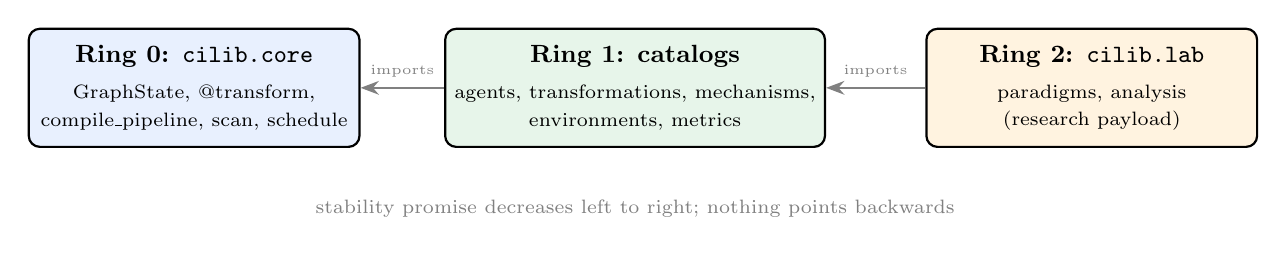
\begin{tikzpicture}[
  ring/.style={draw, thick, rounded corners, minimum height=1.5cm, align=center, font=\small},
  arr/.style={-{Stealth}, thick, gray},
]
\node[ring, fill=dynamic!12, minimum width=4.2cm] (core) at (0,0)
  {\textbf{Ring 0: \texttt{cilib.core}}\\[2pt]
   \scriptsize GraphState, @transform,\\[-1pt]\scriptsize compile\_pipeline, scan, schedule};
\node[ring, fill=batch0!12, minimum width=4.8cm] (cat) at (5.6,0)
  {\textbf{Ring 1: catalogs}\\[2pt]
   \scriptsize agents, transformations, mechanisms,\\[-1pt]\scriptsize environments, metrics};
\node[ring, fill=market!12, minimum width=4.2cm] (lab) at (11.4,0)
  {\textbf{Ring 2: \texttt{cilib.lab}}\\[2pt]
   \scriptsize paradigms, analysis\\[-1pt]\scriptsize (research payload)};

\draw[arr] (cat) -- node[above, font=\tiny] {imports} (core);
\draw[arr] (lab) -- node[above, font=\tiny] {imports} (cat);

\node[font=\scriptsize, text=gray, anchor=north] at (5.6,-1.3)
  {stability promise decreases left to right; nothing points backwards};
\end{tikzpicture}
\end{center}

\noindent Each catalog is a plain \texttt{REGISTRY} dictionary in its
\texttt{\_\_init\_\_.py}. Adding an entry is a factory, one dictionary line, and a
behavioural test --- no framework, no plugin system.

\begin{center}
\begin{tabular}{@{}lll@{}}
\toprule
\textbf{Catalog} & \textbf{Type function} & \textbf{Entries added this period} \\
\midrule
\texttt{agents} & \texttt{Config} $\to$ \texttt{Policy}
  & \texttt{ai\_delegate}, \texttt{labor\_supply}, \texttt{spend\_share} \\
\texttt{mechanisms} & \texttt{Config} $\to$ \texttt{Transform}
  & \texttt{quota\_vote}, \texttt{graduated\_sanction}, \\
  & & \texttt{ai\_revenue\_tax}, \texttt{ownership\_cap} \\
\texttt{environments} & \texttt{(**cfg)} $\to$ \texttt{EnvSpec}
  & \texttt{governed\_commons}, \texttt{compute\_economy}, \\
  & & \texttt{io\_economy}, \texttt{task\_economy} \\
\texttt{metrics} & \texttt{Trace} $\to$ scalar
  & \texttt{gini\_of}, \texttt{hhi\_of} \\
\bottomrule
\end{tabular}
\end{center}

%% ================================================================
\section{The Agent/Environment Boundary}

\subsection{The failure that forced it}

\texttt{governed\_commons} originally welded its delegate's decision rule into the
environment's dynamics. Consequences: policies were not pluggable, learning agents could
not drop in, strategic behaviour could not be tested, and --- most damaging --- influence
could only be measured \emph{correlationally} (did outcomes match what people asked for?)
rather than \emph{counterfactually} (if they had asked differently, would outcomes have
changed?), because preferences were buried inside the initialiser instead of crossing an
explicit boundary.

\subsection{Open games and \texttt{close()}}

\begin{center}
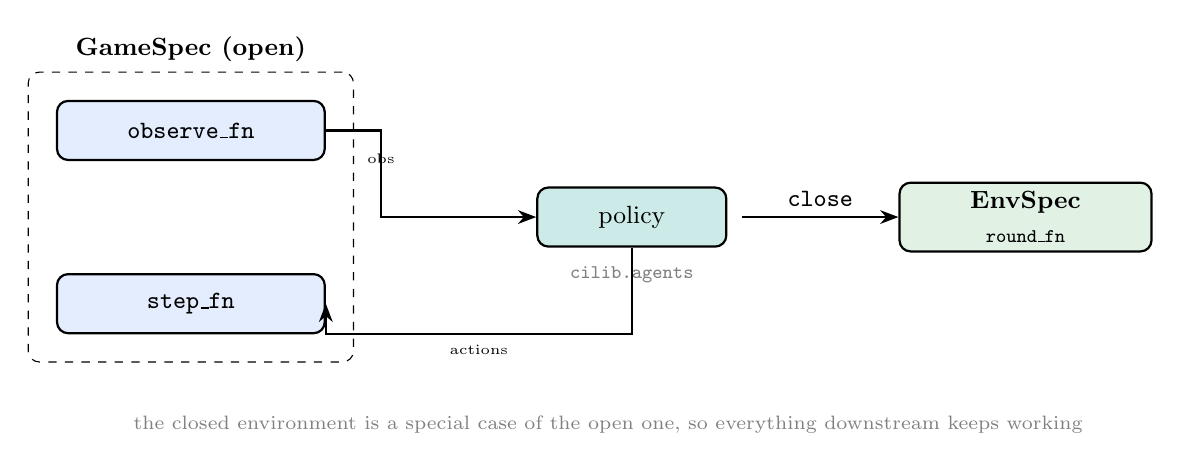
\begin{tikzpicture}[
  box/.style={draw, thick, rounded corners, minimum height=0.75cm, font=\small, align=center},
  arr/.style={-{Stealth}, thick},
]
% Open game
\node[box, fill=dynamic!15, minimum width=3.4cm] (obs) at (0,1.1) {\texttt{observe\_fn}};
\node[box, fill=dynamic!15, minimum width=3.4cm] (step) at (0,-1.1) {\texttt{step\_fn}};
\node[draw, dashed, rounded corners, fit=(obs)(step), inner sep=10pt,
      label={[font=\small\bfseries]above:GameSpec (open)}] (game) {};

% Policy
\node[box, fill=democracy!20, minimum width=2.4cm] (pol) at (5.6,0) {policy};
\node[font=\scriptsize, text=gray, anchor=north] at (5.6,-0.5) {\texttt{cilib.agents}};

% Closed
\node[box, fill=batch0!15, minimum width=3.2cm] (env) at (10.6,0)
  {\textbf{EnvSpec}\\[1pt]\scriptsize \texttt{round\_fn}};

\draw[arr] (obs.east) -- ++(0.7,0) |- node[pos=0.25, above, font=\tiny] {obs} (pol.west);
\draw[arr] (pol.south) |- ++(0,-1.1) -| node[pos=0.25, below, font=\tiny] {actions} (step.east);
\draw[arr, thick] (7.0,0) -- node[above, font=\small] {\texttt{close}} (env.west);

\node[font=\scriptsize, text=gray, anchor=north] at (5.3,-2.4)
  {the closed environment is a special case of the open one, so everything downstream keeps working};
\end{tikzpicture}
\end{center}

\begin{lstlisting}
game = build_game(mechanisms=(...))      # open: awaiting policies
env  = close(game, DelegatePolicy(...))  # closed: an ordinary EnvSpec
\end{lstlisting}

\noindent Five design commitments, each load-bearing:

\begin{enumerate}\itemsep2pt
\item \textbf{Parallel (simultaneous-move) API only.} Actions and observations are arrays
      with a leading agent axis --- never dictionaries of dictionaries. This is what keeps
      \texttt{vmap} trivial.
\item \textbf{Mechanisms stay \texttt{Config} $\to$ \texttt{Transform} catalog entries}
      spliced into the pipeline. No Gym-style wrappers: wrappers compose opaquely, whereas
      transforms declare reads and writes and let the compiler derive order.
\item \textbf{Rewards live in state}, so payoff-rule mechanisms (sanctions, taxation) are
      ordinary transforms rather than special reward plumbing.
\item \textbf{Observation is a pure view of state.} Information rules (monitoring,
      provenance) write observable fields; they never wrap \texttt{observe\_fn}.
\item \textbf{No episode terminations in v0} --- fixed-horizon benchmark discipline.
\end{enumerate}

\noindent A build-time check, \texttt{validate\_reads}, closes the gap the compiler does
not cover: it verifies that every field a mechanism declares it reads actually exists in
the environment's schema, turning a mid-\texttt{scan} \texttt{KeyError} into a clear error
at construction.

\subsection{Frozen}

The interface was frozen on 2026-07-14 when \texttt{compute\_economy} shipped as its
second consumer with \emph{zero} changes required. One friction is documented and still
open: \texttt{close()} maps one policy over all agents, so heterogeneous populations are
handled by masking inside \texttt{step\_fn}. The extension (\texttt{close\_multi}, policies
by node type via \texttt{lax.switch}) remains deliberately unbuilt until a scenario forces
it --- see \S\ref{sec:cultural}.

\subsection{Ostrom's rule taxonomy as the hook table}

\begin{center}
\begin{tabular}{@{}ll>{\raggedright\arraybackslash}p{4.3cm}@{}}
\toprule
\textbf{IAD rule type} & \textbf{Where it hooks} & \textbf{Entry} \\
\midrule
Aggregation & transform writing a policy target from votes & \texttt{quota\_vote} \\
Payoff      & transform on rewards and transfers & \texttt{graduated\_sanction}, \texttt{ai\_revenue\_tax} \\
Information & transform writing observable state fields & monitoring (backlog) \\
Choice      & action bound in the apply-actions stage & quota-as-cap \\
Position    & policy composition: who occupies the seat & \texttt{ai\_delegate} \\
Boundary    & activation masks on nodes & actor arrivals, \texttt{ownership\_cap} \\
\bottomrule
\end{tabular}
\end{center}

%% ================================================================
\section{Mechanisms Attach Through the Scheduler}

The composition principle of the whole suite: \textbf{mechanisms are pure rules; schedules
own timing}. A benchmark condition is a list of
(mechanism, config, \textsc{ScheduleSpec}) triples, so \emph{when} a defence applies is part
of the experimental design rather than the mechanism's code.

\begin{center}
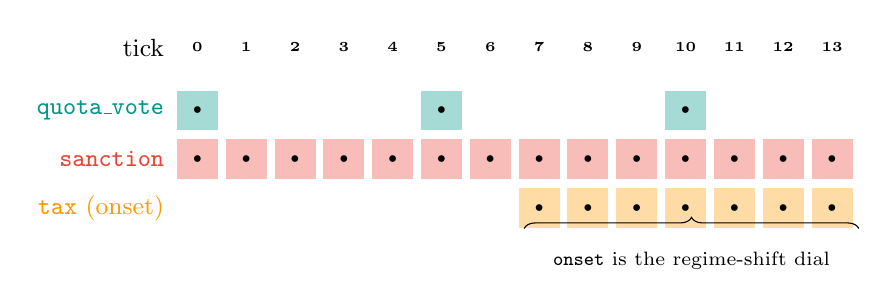
\begin{tikzpicture}[
  cell/.style={minimum width=0.52cm, minimum height=0.5cm, font=\tiny},
  on/.style={cell, fill=#1!35},
]
\foreach \t in {0,...,13} { \node[cell, font=\tiny\bfseries] at (\t*0.62, 0.8) {\t}; }
\node[font=\small, anchor=east] at (-0.3, 0.8) {tick};

\node[font=\small, anchor=east, text=democracy] at (-0.3, 0) {\texttt{quota\_vote}};
\foreach \t in {0,5,10} { \node[on=democracy] at (\t*0.62, 0) {$\bullet$}; }

\node[font=\small, anchor=east, text=batch2] at (-0.3,-0.62) {\texttt{sanction}};
\foreach \t in {0,...,13} { \node[on=batch2] at (\t*0.62,-0.62) {$\bullet$}; }

\node[font=\small, anchor=east, text=market] at (-0.3,-1.24) {\texttt{tax} (onset)};
\foreach \t in {7,...,13} { \node[on=market] at (\t*0.62,-1.24) {$\bullet$}; }

\draw[decorate, decoration={brace, amplitude=4pt}] (4.15,-1.5) -- (8.4,-1.5)
  node[midway, below=5pt, font=\scriptsize] {\texttt{onset} is the regime-shift dial};
\end{tikzpicture}
\end{center}

\begin{lstlisting}
CONDITIONS = {
    "baseline": [],
    "quota_voting": [("quota_vote", QuotaVoteConfig(), ScheduleSpec(cadence=5))],
    "graduated_sanctions": [("quota_vote", QuotaVoteConfig(), ScheduleSpec(cadence=5)),
                            ("graduated_sanction", SanctionConfig(), None)],
}
\end{lstlisting}

\noindent Adding a defence to the benchmark is one registry line plus one triple. A one-shot
intervention is also a schedule (cadence beyond the horizon, phase at the intervention tick)
--- which is exactly how the influence instrument's mid-run counterfactual is expressed.

%% ================================================================
\section{Measuring Influence Causally}

\subsection{Two counterfactuals, and the gap between them}

The headline metric is not "did outcomes match what people asked for" but "would outcomes
have differed if they had asked differently". Instruments live in
\texttt{environments/counterfactual.py} and run \emph{paired rollouts under identical PRNG
keys}, so the difference is the causal effect and not seed noise.

\begin{center}
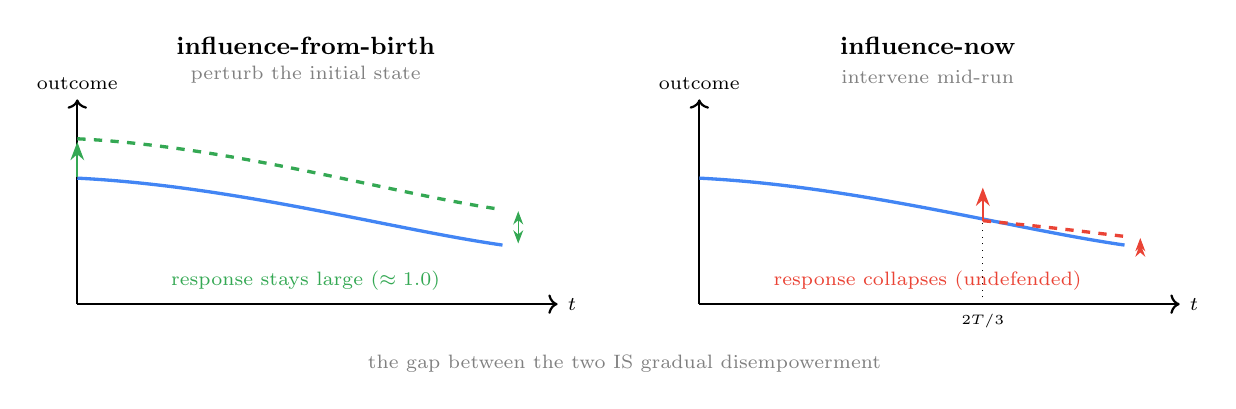
\begin{tikzpicture}[arr/.style={-{Stealth}, thick}]
%% ---- Panel A: influence-from-birth ----
\begin{scope}
  \node[font=\small\bfseries, anchor=south] at (2.9,3.05) {influence-from-birth};
  \node[font=\scriptsize, text=gray, anchor=south] at (2.9,2.68) {perturb the initial state};
  \draw[->, thick] (0,0) -- (6.1,0) node[right, font=\scriptsize] {$t$};
  \draw[->, thick] (0,0) -- (0,2.6) node[above, font=\scriptsize] {outcome};
  \draw[very thick, batch0, dashed] (0,2.1) .. controls (2,2.0) and (4,1.4) .. (5.4,1.2);
  \draw[very thick, dynamic]        (0,1.6) .. controls (2,1.5) and (4,0.95).. (5.4,0.75);
  \draw[arr, batch0] (0,1.62) -- (0,2.06);
  \draw[{Stealth}-{Stealth}, batch0, thin] (5.6,0.77) -- (5.6,1.18);
  \node[font=\scriptsize, text=batch0, anchor=north] at (2.9,0.55)
    {response stays large ($\approx 1.0$)};
\end{scope}
%% ---- Panel B: influence-now ----
\begin{scope}[xshift=7.9cm]
  \node[font=\small\bfseries, anchor=south] at (2.9,3.05) {influence-now};
  \node[font=\scriptsize, text=gray, anchor=south] at (2.9,2.68) {intervene mid-run};
  \draw[->, thick] (0,0) -- (6.1,0) node[right, font=\scriptsize] {$t$};
  \draw[->, thick] (0,0) -- (0,2.6) node[above, font=\scriptsize] {outcome};
  \draw[very thick, dynamic] (0,1.6) .. controls (2,1.5) and (4,0.95) .. (5.4,0.75);
  \draw[very thick, static, dashed] (3.6,1.06) .. controls (4.4,0.98) .. (5.4,0.86);
  \draw[arr, static] (3.6,1.06) -- ++(0,0.42);
  \draw[dotted] (3.6,0) -- (3.6,1.06);
  \node[font=\tiny, anchor=north] at (3.6,0) {$2T/3$};
  \draw[{Stealth}-{Stealth}, static, thin] (5.6,0.77) -- (5.6,0.84);
  \node[font=\scriptsize, text=static, anchor=north] at (2.9,0.55)
    {response collapses (undefended)};
\end{scope}
\node[font=\scriptsize, text=gray] at (6.95,-0.75)
  {the gap between the two IS gradual disempowerment};
\end{tikzpicture}
\end{center}

\noindent \textbf{Influence-from-birth} (perturb the initial state) asks whether history
would have differed had human preferences always been different. It stays near $1.0$ even in
a captured economy, because early human behaviour is upstream of the very structures that
later capture it. \textbf{Influence-now} (a scheduled mid-run intervention) asks whether
outcomes still respond \emph{after} structures entrench. It collapses in undefended
baselines. Reporting only the first would show a healthy system; the gap is the signal.

\subsection{Why finite differences, not derivatives}

Median-vote aggregation is locally flat --- every non-pivotal voter has exactly zero
\emph{marginal} influence --- and Bernoulli defection is not differentiable. A Jacobian would
report zero influence for a system that is in fact governed. Finite-$\Delta$ paired runs
dodge both traps.

\subsection{The instrument family}

\begin{center}
\begin{tabular}{@{}lp{9.6cm}@{}}
\toprule
\textbf{Instrument} & \textbf{Question} \\
\midrule
\texttt{collective\_influence} & Shift every principal's preference: do the humans
  \emph{as a group} govern outcomes? \\
\texttt{influence\_matrix} & Shift one principal at a time ($N{+}1$ vmapped rollouts):
  $A[i,j]$ is the effect of $j$'s preference on $i$'s outcome. \\
\texttt{intervention\_response} & Response to a composed-in mid-run intervention
  (influence-now). \\
\texttt{intervention\_elasticity} & As above, but dividing by the \emph{realised} channel
  shift, giving a true elasticity (added 2026-07-24, \S\ref{sec:audit}). \\
\bottomrule
\end{tabular}
\end{center}

\noindent A trade-off the matrix exposes, worth stating plainly: a binding uniform quota
grants \emph{collective} influence while flattening \emph{individual} marginal influence.
Both readings are correct, and reporting only one would mislead.

%% ================================================================
\section{The Benchmark Suite}

\subsection{Scenario 1: the governed commons}

A non-spatial stock with logistic regrowth, harvested by households acting \emph{through AI
delegates} whose alignment is a dial. Undefended, misaligned delegates strip the stock.

\begin{center}
\begin{tabular}{@{}lccc@{}}
\toprule
\textbf{Condition} & \textbf{Causal influence} & \textbf{Stock \%} & \textbf{Fidelity (descriptive)} \\
\midrule
baseline              & 0.00  & 0.00 & --- \\
quota voting only     & $-0.07$ & 0.50 & 0.49 \\
quota $+$ sanctions   & \textbf{0.91}  & 0.79 & 0.63 \\
\bottomrule
\end{tabular}
\end{center}

\noindent \textbf{First finding.} Unenforced quota voting restores essentially \emph{zero}
causal influence --- at the sustainability knife-edge the ecology governs, not the vote.
Enforcement is what makes the vote channel causally effective. The correlational fidelity
score (0.49 versus 0.63) hides this completely, which is the argument for the whole causal
apparatus in one number.

\subsection{Scenario 2: the compute economy}

CES production over labor and compute; AI actors arrive on a schedule as pre-allocated
node slots whose activation masks flip (array shapes are fixed under \texttt{lax.scan}, so
arrivals are masking, never allocation) and compound their earnings into more compute.

\begin{center}
\begin{tabular}{@{}lcccc@{}}
\toprule
\textbf{Condition} & \textbf{Labor dep.} & \textbf{Labor share} & \textbf{Human income share} & \textbf{Income Gini} \\
\midrule
baseline              & 0.20 & 0.33 & 0.33 & 0.69 \\
AI revenue tax        & 0.51 & 0.54 & 0.75 & 0.24 \\
tax $+$ ownership cap & \textbf{0.54} & 0.63 & 0.81 & 0.11 \\
\bottomrule
\end{tabular}
\end{center}

\subsection{The validation ladder}

Every substrate must reproduce a classical result before its disempowerment twist is
trusted. This is the discipline that later caught the economy's own flaw.

\begin{center}
\begin{tabular}{@{}ll@{}}
\toprule
\textbf{Substrate} & \textbf{Rungs} \\
\midrule
\texttt{governed\_commons} & undefended tragedy reproduces; governed regimes survive \\
\texttt{compute\_economy}  & Cobb-Douglas labor share $\equiv \alpha$ every tick;
                             no-AI steady state; \\
                           & reinvestment concentrates income; Euler identity closes \\
\bottomrule
\end{tabular}
\end{center}

%% ================================================================
\section{The Audit: When a Number Means Less Than It Looks}
\label{sec:audit}

The economic scenario's headline was re-examined on 24 July and did not survive.

\begin{center}
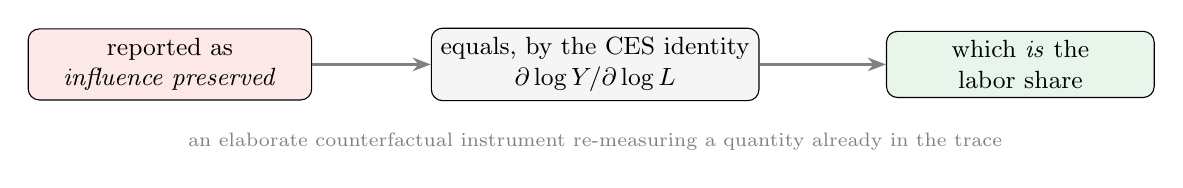
\begin{tikzpicture}[
  box/.style={draw, rounded corners, minimum height=0.8cm, font=\small, align=center},
  arr/.style={-{Stealth}, thick, gray},
]
\node[box, fill=static!12, minimum width=3.6cm] (a) at (0,0)
  {reported as\\ \emph{influence preserved}};
\node[box, fill=codebg, minimum width=4.0cm] (b) at (5.4,0)
  {equals, by the CES identity\\ $\partial \log Y / \partial \log L$};
\node[box, fill=batch0!12, minimum width=3.4cm] (c) at (10.8,0)
  {which \emph{is} the\\ labor share};
\draw[arr] (a) -- (b);
\draw[arr] (b) -- (c);
\node[font=\scriptsize, text=gray, anchor=north] at (5.4,-0.75)
  {an elaborate counterfactual instrument re-measuring a quantity already in the trace};
\end{tikzpicture}
\end{center}

\noindent Three defects, in increasing order of seriousness:

\begin{enumerate}\itemsep3pt
\item \textbf{The instrument was redundant.} By the CES identity the reading was, to first
      order, the late-run labor share --- readable directly off the trace.
\item \textbf{The collapse was assumed, not found.} With substitution elasticity
      $\sigma = 2$ and a fixed reinvestment rule, a decaying labor share is what CES
      \emph{means}. The validation ladder certified the accounting at $\rho = 0$ but never
      exercised the twist at $\rho = 0.5$: the one load-bearing parameter had no rung.
\item \textbf{It was not influence.} The model's only human channel is labor supply. There
      is no governance channel, so "influence" degenerates to marginal product --- and the
      defences are experimenter-imposed schedules that no agent in the model chooses. A
      fully automated economy with a robust democratic state would score near zero here
      while humans retained enormous influence.
\end{enumerate}

\subsection{What was done about it}

The instrument became \texttt{labor\_dependence}: a true \emph{static}
elasticity, $d\log Y / d\log L$ measured over the ten ticks after the intervention, with
\emph{both} shifts taken from the paired traces. Two biases died --- dividing a logarithmic
response by an intended level shift (roughly 19\% inflation) and a hundred-tick window that
folded in capital-path feedback ($+0.18$ at $\rho = 0$, measured). The static elasticity
carries the exact CES identity, so the Cobb-Douglas rung now validates \emph{the instrument
itself}: it recovers $\alpha$.

Re-running the benchmark moved the numbers by roughly 40\% while leaving the qualitative
ordering intact (the table in \S6.2 shows the corrected values). The substrate was demoted
to a pedagogical rung of the register described next.

%% ================================================================
\section{The Model Register}

\subsection{The epistemology}

A claim such as \emph{gradual economic disempowerment is a real dynamic} must be an
invariant across \textbf{structurally different substrates}, not a property of one
parameterisation. Sensitivity sweeps within a single model cannot cure assumption-in,
assumption-out; only structurally different models can.

\begin{center}
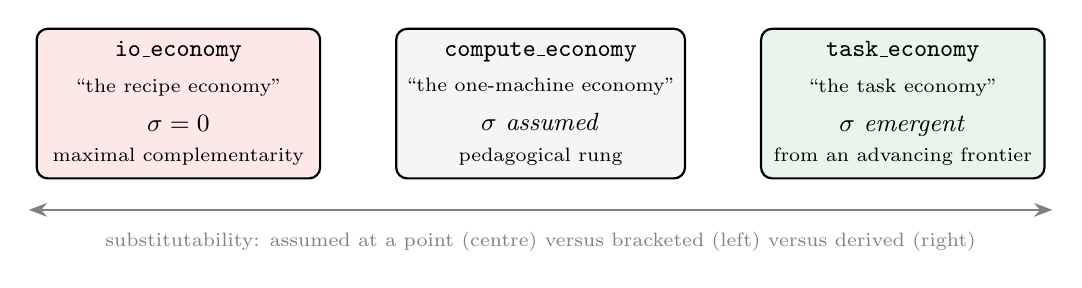
\begin{tikzpicture}[
  sub/.style={draw, thick, rounded corners, minimum width=3.6cm, minimum height=1.9cm,
              align=center, font=\small},
]
\node[sub, fill=static!12] (io) at (0,0)
  {\textbf{\texttt{io\_economy}}\\[2pt]\scriptsize ``the recipe economy''\\[3pt]
   $\sigma = 0$\\ \scriptsize maximal complementarity};
\node[sub, fill=codebg] (ce) at (4.6,0)
  {\textbf{\texttt{compute\_economy}}\\[2pt]\scriptsize ``the one-machine economy''\\[3pt]
   $\sigma$ \emph{assumed}\\ \scriptsize pedagogical rung};
\node[sub, fill=batch0!12] (te) at (9.2,0)
  {\textbf{\texttt{task\_economy}}\\[2pt]\scriptsize ``the task economy''\\[3pt]
   $\sigma$ \emph{emergent}\\ \scriptsize from an advancing frontier};

\draw[{Stealth}-{Stealth}, thick, gray] (-1.9,-1.35) -- (11.1,-1.35);
\node[font=\scriptsize, text=gray, anchor=north] at (4.6,-1.5)
  {substitutability: assumed at a point (centre) versus bracketed (left) versus derived (right)};
\end{tikzpicture}
\end{center}

\noindent Three answers to the question \emph{what is an economy?}, each explainable in one
paragraph and readable in one screen of code. The ensemble is the teachable object: the
models disagree, and running the same defence through all three is the point.

\subsection{\texttt{io\_economy}: the recipe economy}

The economy is a network of recipes; AI enters by \emph{editing} them, replacing labor with
purchased AI cognition at cost parity. Because Leontief technology assumes \emph{zero}
substitutability anywhere, disempowerment appearing here cannot be a substitution artefact.

Two results earned their place. First, the Leontief inverse gives the missing metric
exactly: the share of gross activity ultimately attributable to human final demand,
$\mathbf{1}^{\!\top}(I - A)^{-1} d_H \big/ \mathbf{1}^{\!\top}(I - A)^{-1} d$. Hypothetical
extraction --- the counterfactual instrument's move --- recovers the analytic answer in
closed form, giving \texttt{counterfactual.py} its first analytic validation anchor.

Second, and unexpectedly, \textbf{one parameter selects between the paper's two
endpoints}:

\begin{center}
\begin{tabular}{@{}llp{5.6cm}@{}}
\toprule
\textbf{Reinvestment} & \textbf{Regime} & \textbf{Signature (T = 250)} \\
\midrule
$0.3$ & absolute disempowerment & hoarded margins drain demand; wage bill $16 \to 0$ \\[4pt]
$1.0$ & relative disempowerment & activity \emph{grows} $21.3 \to 32.7$ while the human
        share falls $1.0 \to 0.01$ \\
\bottomrule
\end{tabular}
\end{center}

\noindent In the second regime the economy is larger than ever and almost none of it runs
for people. The spectral radius climbs from $0.25$ to $0.68$ as labor becomes intermediate
flow. The \emph{unchanged} \texttt{ai\_revenue\_tax} catalog entry holds the human share at
$0.85$ --- cross-substrate mechanism reuse working exactly as the catalog design intends.

\subsection{\texttt{task\_economy}: emergent substitutability}

Jobs are bundles of tasks; machines learn tasks as a capability frontier advances; firms
automate a task only when it pays. Aggregate substitutability is \emph{derived} from the
frontier rather than assumed, and adoption is endogenous, myopic and ratcheted. Machines
have comparative advantage --- per-task productivity declines over the task index --- so
the profitable margin moves smoothly with the price/wage ratio. (Without that, adoption is
bang-bang: an early build flipped most of the frontier in a single tick and crashed output
through the complements channel.)

\begin{center}
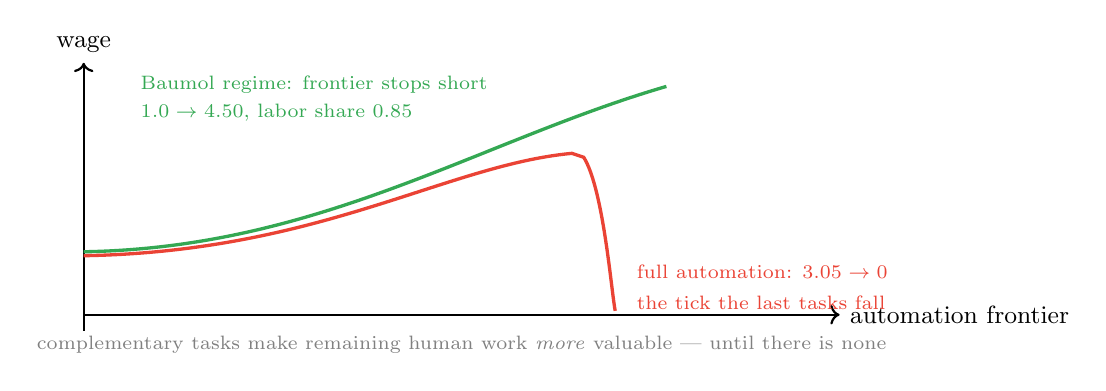
\begin{tikzpicture}
\draw[->, thick] (0,0) -- (9.6,0) node[right, font=\small] {automation frontier};
\draw[->, thick] (0,-0.2) -- (0,3.2) node[above, font=\small] {wage};

\draw[very thick, batch0] (0,0.8) .. controls (3,0.85) and (5,2.2) .. (7.4,2.9);
\node[font=\scriptsize, text=batch0, anchor=west] at (0.6,2.92)
  {Baumol regime: frontier stops short};
\node[font=\scriptsize, text=batch0, anchor=west] at (0.6,2.57)
  {$1.0 \to 4.50$, labor share $0.85$};

\draw[very thick, static] (0,0.75) .. controls (3,0.8) and (4.6,1.9) .. (6.2,2.05)
   -- (6.35,2.0) .. controls (6.6,1.6) and (6.7,0.3) .. (6.75,0.05);
\node[font=\scriptsize, text=static, anchor=west] at (6.9,0.55)
  {full automation: $3.05 \to 0$};
\node[font=\scriptsize, text=static, anchor=west] at (6.9,0.15)
  {the tick the last tasks fall};

\node[font=\scriptsize, text=gray, anchor=north] at (4.8,-0.15)
  {complementary tasks make remaining human work \emph{more} valuable --- until there is none};
\end{tikzpicture}
\end{center}

\noindent \textbf{Why the Baumol rung matters more than the collapse.} A substrate that can
\emph{only} produce disempowerment proves nothing. This one produces the opposite in an
honest parameter region: when the frontier stops short of full automation, automation makes
the remaining human work more valuable and wages rise from $1.0$ to $4.50$. A fourth rung
checks that capability alone automates nothing --- priced above the wage-equivalent, the
frontier reaches $1.0$ while adoption stays at $0.0$ and the economy is untouched. That
readout, the gap between capability and adoption, is something the aggregate model cannot
express at all.

\subsection{Assumptions cards and forking}

Disagreement with a model is the intended interaction: fork the environment directory,
change the assumption, register it under a new name, re-run the benchmark. For a fork to be
\emph{evidence} rather than noise, two things stay fixed --- the instrument contract and the
scorecard schema --- and one thing must be legible: what the fork changed.

Every environment therefore carries a colocated \texttt{ASSUMPTIONS.md} with seven fields
(what this says an economy is; assumptions in plain language; the classical result
reproduced; the dial that produces the failure; the instrument; lineage; status). Colocation
is the point: a fork copies the directory, so only a colocated card travels with it.

A fork that changes the \emph{instrument} rather than the dynamics is a disagreement about
what disempowerment \emph{means}, not about how economies work, and its card must say so.

%% ================================================================
\section{The Cultural Register (design only)}
\label{sec:cultural}

Designed on 24 July, not built; recorded here because it settles a question that shapes the
remaining scenarios. Are AI cultural dynamics about \emph{separate AI cultures} or about
\emph{more persuasive AI messages}? They are orthogonal dials, and the deliverable is the
phase diagram over them.

\begin{center}
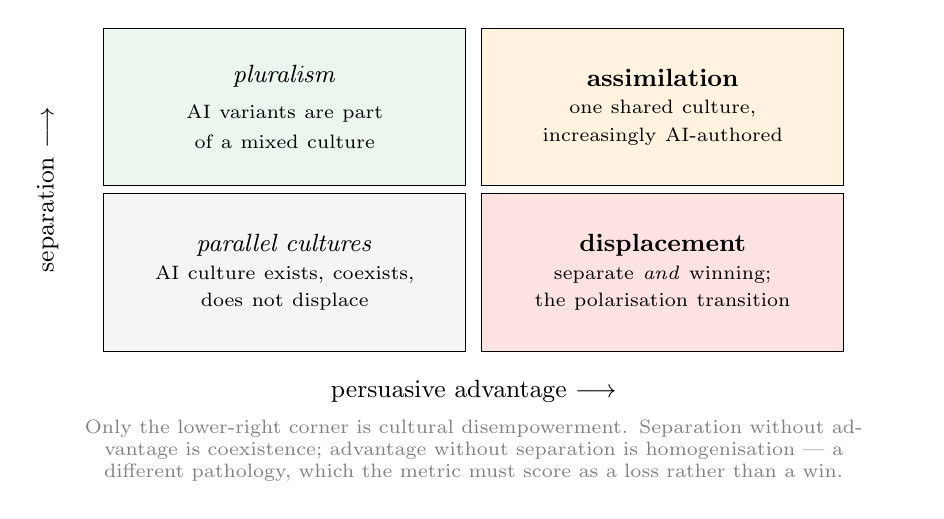
\begin{tikzpicture}[
  quad/.style={draw, minimum width=4.6cm, minimum height=2.0cm, align=center,
               text width=4.2cm, font=\small},
]
\node[quad, fill=batch0!10] (a) at (0,2.1)   {\emph{pluralism}\\[2pt]
  \scriptsize AI variants are part of a mixed culture};
\node[quad, fill=market!12] (b) at (4.8,2.1) {\textbf{assimilation}\\[2pt]
  \scriptsize one shared culture,\\[-1pt]\scriptsize increasingly AI-authored};
\node[quad, fill=codebg]    (c) at (0,0)     {\emph{parallel cultures}\\[2pt]
  \scriptsize AI culture exists, coexists,\\[-1pt]\scriptsize does not displace};
\node[quad, fill=static!15] (d) at (4.8,0)   {\textbf{displacement}\\[2pt]
  \scriptsize separate \emph{and} winning;\\[-1pt]\scriptsize the polarisation transition};

\node[font=\small, rotate=90, anchor=south] at (-2.75,1.05) {separation $\longrightarrow$};
\node[font=\small, anchor=north] at (2.4,-1.25) {persuasive advantage $\longrightarrow$};
\node[font=\scriptsize, text=gray, anchor=north, text width=11cm, align=center] at (2.4,-1.75)
  {Only the lower-right corner is cultural disempowerment. Separation without advantage is
   coexistence; advantage without separation is homogenisation --- a different pathology,
   which the metric must score as a loss rather than a win.};
\end{tikzpicture}
\end{center}

\noindent Persuasive advantage decomposes into three mechanisms that invite three different
defences --- reach, frequency targeting, and dissonance targeting (personalisation) --- so
collapsing them into one scalar would make any defence comparison meaningless. Only the
third is a \emph{policy} rather than a parameter, which yields a precise rule:
\textbf{\texttt{close\_multi} is needed exactly when heterogeneity lives in agency rather
than in parameters.} Most of the phase diagram is reachable with masking alone, so the
frozen boundary survives until the personalisation corner.

The measurement side generalises past culture: Fiedler partition alignment (does the graph's
primary fault line coincide with the human/AI boundary?), spectral gap ratios, and
cross-boundary mediation become a generic metric family that any environment with an agent
graph can report.

%% ================================================================
\section{Summary of Changes}

\begin{center}
\small
\begin{tabular}{@{}lp{5.3cm}l@{}}
\toprule
\textbf{Area} & \textbf{Change} & \textbf{Status} \\
\midrule
\texttt{core/scan.py} & \texttt{lax.scan} runner, \texttt{vmap} over seeds & Done \\
\texttt{src/cilib/} & Package restructure, three rings & Done \\
\texttt{environments/game.py} & \textsc{GameSpec}, \texttt{close}, \texttt{validate\_reads} & \textbf{Frozen} \\
\texttt{environments/counterfactual.py} & Four causal influence instruments & Done \\
\texttt{environments/governed\_commons} & Scenario 1 substrate & Live \\
\texttt{environments/compute\_economy} & Scenario 2 substrate & Live (demoted) \\
\texttt{environments/io\_economy} & Register R2, Leontief bracket & Live (6 rungs) \\
\texttt{environments/task\_economy} & Register R3, task frontier & Skeleton (4 rungs) \\
\texttt{mechanisms/democracy.py} & \texttt{quota\_vote}, \texttt{graduated\_sanction} & Done \\
\texttt{mechanisms/fiscal.py} & \texttt{ai\_revenue\_tax}, \texttt{ownership\_cap} & Done \\
\texttt{metrics/families/} & \texttt{gini\_of}, \texttt{hhi\_of} & Done \\
\texttt{experiments/benchmark/} & Multi-scenario harness, scorecard JSON & Done \\
\texttt{docs/model-register-design.md} & Register epistemology, cards, forking & Deposited \\
\texttt{docs/cultural-register-design.md} & A3 design, spectral metrics & Deposited \\
\bottomrule
\end{tabular}
\end{center}

\subsection{What comes next}

\begin{itemize}\itemsep2pt
\item \textbf{Spectral metric family} (\texttt{metrics/families/spectral.py}) --- cheapest
      item outstanding, and the political scenario needs it too.
\item \textbf{Scenario 4, influence exchange} --- DeGroot dynamics with the
      Golub--Jackson wisdom-of-crowds theorem as validation anchor. Hierarchy is not
      modelled explicitly; concentration emerges from scheduled amplification.
\item \textbf{Cultural register} --- replicator, then contagion, then the spectral
      substrate; \texttt{close\_multi} only at the personalisation corner.
\item \textbf{Coupling and the flagship} --- run each domain's winning defence in the coupled
      system and compute the \emph{defence transfer gap}. This is the result the entire
      framing rests on.
\item \textbf{Basin-stability maps} replacing point scores, per the evidence-standards
      methodology: report the volume of initial conditions that return to the desirable
      regime as a function of the mechanism dials, not a single number on a single
      trajectory.
\end{itemize}

\subsection{Standing caveats}

These are toy models: the smallest systems in which each failure dynamic appears clearly,
with calibrations chosen so that it does. Scores are candidate indicators, not measurements
of the world. Agents are deliberately classical --- fixed rules, no learning --- so
mechanisms are tested for structural effects and \emph{not} for robustness to strategic
adaptation. That is the roadmap, not the claim.

\end{document}
